\documentclass[letterpaper, 12pt]{article}

%%%%%%%%%%%%%%%%%%%%%%%%%%%%%
% DEFINITIONS
% Change those informations
% If you need umlauts you have to escape them, e.g. for an ü you have to write \"u
\gdef\mytitle{Ausarbeitung}
\gdef\mythema{Zahlungssyteme}

\gdef\mysubject{Ethik}
\gdef\mycourse{5BHIT 2017/18}
\gdef\myauthor{Martin W\"olfer, Johannes Bishara}

\gdef\myversion{0.1}
\gdef\mybegin{Begonnen am 19. November 2017}
\gdef\myfinish{Beendet am 19. November}

\gdef\mygrade{Note:}
\gdef\myteacher{Betreuer: GRAFM}
%
%%%%%%%%%%%%%%%%%%%%%%%%%%%%%

%!TEX root=../document.tex

\usepackage[in]{fullpage}
% Fontencoding for possible copy&paste out of PDF
\usepackage[T1]{fontenc}
\usepackage[utf8]{inputenc}
\usepackage[ngerman]{babel}
\usepackage{graphicx} 
\usepackage{wasysym}
\usepackage{textcomp}
\usepackage{sectsty}
\usepackage{caption}
\usepackage{listings}
\usepackage{array}
\usepackage{nonfloat}
\usepackage{colortbl}
\usepackage{footmisc}
\usepackage{fancyhdr}
\usepackage{ccicons}
\usepackage{suffix}
\usepackage{multirow}
\usepackage{tabularx}
\usepackage{listings}
\usepackage{accsupp}
\usepackage{color}
\usepackage{url}
\usepackage[dvipsnames]{xcolor}
\usepackage[longnamesfirst,nonamebreak]{natbib}
\usepackage[headsep=1cm,headheight=3cm,hmargin=2cm,vmargin=2.5cm]{geometry}
\usepackage[nolist]{acronym}

% Definitions for Textcolor
\usepackage{color}
\definecolor{listings}{rgb}{0.96, 0.96, 0.96}
\definecolor{update}{rgb}{1, 0.8, 0.8}
\definecolor{config}{rgb}{0.8, 1, 0.8}
\definecolor{gray}{rgb}{0.4,0.4,0.4}
\definecolor{darkblue}{rgb}{0.0,0.0,0.6}
\definecolor{cyan}{rgb}{0.0,0.6,0.6}

% Java Syntaxhighligthning
% strings
\definecolor{javared}{rgb}{0.6,0,0}
% comments
\definecolor{javagreen}{rgb}{0.25,0.5,0.35}
% keywords
\definecolor{javapurple}{rgb}{0.5,0,0.35}
% javadoc
\definecolor{javadocblue}{rgb}{0.25,0.35,0.75}

\lstset{
	basicstyle=\ttfamily\small,
	keywordstyle=\bfseries\color[rgb]{0.496,0.000,0.332},
	commentstyle=\color[rgb]{0.246,0.496,0.371},
	stringstyle=\color[rgb]{0.164,0.000,0.996},
	tabsize=4,
	breaklines=true,
	numbers=left,
	numberstyle=\tiny\color{black},
	stepnumber=2,
	numbersep=8pt,
	numberstyle=\tiny,
	captionpos=b,
	xleftmargin=1cm,
	showspaces=false,
	showstringspaces=false,
	basewidth={0.53em,0.45em},
	frame=single,
	xleftmargin=1cm,
	basicstyle=\scriptsize,
}


\lstdefinestyle{Java}{
	language=Java,
	keywordstyle=\color{javapurple}\bfseries,
	stringstyle=\color{javared},
	commentstyle=\color{javagreen},
	morecomment=[s][\color{javadocblue}]{/**}{*/},
}

\lstdefinelanguage{XML}
{
	morestring=[b]",
	morestring=[s]{>}{<},
	morecomment=[s]{<?}{?>},
	stringstyle=\color{black},
	identifierstyle=\color{darkblue},
	keywordstyle=\color{cyan},
	% list your attributes here
	morekeywords={xmlns,version,type}
}

\lstdefinestyle{XML}{
	language=XML,
	basicstyle=\ttfamily\small,
	columns=fullflexible,
	commentstyle=\color{gray}\upshape
}

\newcommand{\noncopynumber}[1]{
	\BeginAccSupp{method=escape,ActualText={}}
	#1
	\EndAccSupp{}
}
\lstdefinestyle{bash}{
	language=bash,
	basicstyle=\ttfamily\small,
	literate={-}{{-}}{1},
	% http://tex.stackexchange.com/questions/145416/how-to-have-straight-single-quotes-in-lstlistings
	upquote=true;
	showstringspaces=false,
	%numbers=none,
	% http://tex.stackexchange.com/questions/122256/only-select-code-without-line-numbers
	numberstyle=\tiny\noncopynumber,
	breaklines=false,
	columns=fullflexible,
	basicstyle=\scriptsize
}

% http://tex.stackexchange.com/questions/83085/how-to-improve-listings-display-of-json-files
\colorlet{punct}{red!60!black}
\definecolor{background}{HTML}{EEEEEE}
\definecolor{delim}{RGB}{20,105,176}
\colorlet{numb}{magenta!60!black}
\lstdefinelanguage{json}{
	basicstyle=\ttfamily\small,
	numbers=left,
	numberstyle=\scriptsize,
	stepnumber=2,
	numbersep=8pt,
	showstringspaces=false,
	breaklines=true,
	literate=
	*{0}{{{\color{numb}0}}}{1}
	{1}{{{\color{numb}1}}}{1}
	{2}{{{\color{numb}2}}}{1}
	{3}{{{\color{numb}3}}}{1}
	{4}{{{\color{numb}4}}}{1}
	{5}{{{\color{numb}5}}}{1}
	{6}{{{\color{numb}6}}}{1}
	{7}{{{\color{numb}7}}}{1}
	{8}{{{\color{numb}8}}}{1}
	{9}{{{\color{numb}9}}}{1}
	{:}{{{\color{punct}{:}}}}{1}
	{,}{{{\color{punct}{,}}}}{1}
	{\{}{{{\color{delim}{\{}}}}{1}
	{\}}{{{\color{delim}{\}}}}}{1}
	{[}{{{\color{delim}{[}}}}{1}
	{]}{{{\color{delim}{]}}}}{1},
	basicstyle=\scriptsize
}

\usepackage[
	colorlinks,
	citecolor=black,
	filecolor=black,
	linkcolor=black,
	urlcolor=black,
	linktoc=all
]{hyperref}


\let\tempsection\section
\renewcommand\section[1]{\vspace{-0.3cm}\tempsection{#1}\vspace{-0.3cm}}
\WithSuffix\newcommand\section*[1]{\tempsection*{#1}}

\let\tempsubsection\subsection
\renewcommand\subsection[1]{\vspace{0cm}\tempsubsection{#1}\vspace{0cm}}

\let\tempsubsubsection\subsubsection
\renewcommand\subsubsection[1]{\vspace{0cm}\tempsubsubsection{#1}\vspace{0cm}}

\linespread{0.94}

\lhead{\mysubject}
\chead{}
\rhead{\bfseries\mythema}
\lfoot{\mycourse}
\cfoot{\thepage}
% Creative Commons license BY
% http://creativecommons.org/licenses/?lang=de
\rfoot{\ccby\hspace{2mm}\myauthor}
\renewcommand{\headrulewidth}{0.4pt}
\renewcommand{\footrulewidth}{0.4pt}

\begin{document}
	\parindent 0pt
	\parskip 6pt
	
	\pagenumbering{Roman} 
	%!TEX root=../laborprotokoll.tex

\begin{titlepage}

	\begin{figure}[!h]
		\begin{flushright}
			
\includegraphics[width=0.3\linewidth]{images/jdIT_tgm.png}
		\end{flushright}
	\end{figure}

	\vspace{2.5cm} 

	{\begin{center} \bfseries\huge
			\rule{17.5cm}{0.1mm}  
			\\[5mm]
			\mytitle\\[5mm]
			\mythema\\
			\rule{17.5cm}{0.1mm}  
	\end{center}}

	{\begin{flushright} \bfseries\Large
			\vspace{2cm}
			\mysubject\\
			\mycourse\\[10mm]
			\myauthor\\[10mm]
	\end{flushright}}

	{\begin{table}[!h] \bfseries\normalsize
		\begin{tabularx}{\textwidth}{lXr @{\hspace{0mm}}}
			&& Version \myversion\\
			\mygrade && \mybegin\\
			\myteacher && \myfinish\\
		\end{tabularx}
	\end{table}}

\end{titlepage}

	
	\clearpage
	\thispagestyle{empty}
	\tableofcontents
	
	\newpage
	\pagenumbering{arabic}
	\pagestyle{fancy}
	
	%\vspace{-0.5cm}
	
	%!TEX root=../document.tex

\section{Allgemein}
\subsection{Definition}
\textit{\textbf{Als Zahlungsverfahren werden alle Formen und Prozesse der Übertragung von Eigentumsrechten an Zahlungsmitteln bezeichnet.}}

Andere Bezeichnungen: \textbf{Bezahlverfahren}, \textbf{Zahlungssysteme}, \textbf{Zahlungsinstrumente}.

\subsection{Klassifizierungen}
\subsection{Klassisch vs Elektronisch}
Oft wird in \textbf{elektronische} und \textbf{klassische} Zahlungssysteme unterschieden, beispielsweise stellen Zahlungsarten wie Nachnahme, Scheck oder Überweisung ein klassisches Zahlungssystem dar. Wichtig dabei ist, dass die Rechnung \textbf{vor} oder \textbf{nach} der Bestellung bzw. Lieferung erfolgt. 

Bei elektronischen Zahlungssysteme erfolgt die Zahlung unmittelbar über elektronische Medien. Beispiele dafür wären Kreditkartenzahlungen, Bankomatzahlungen, Lastschriftzahlungen. 

Diese Unterscheidung weist jedoch einige Probleme auf, unter anderem ist das unabdingbare \textbf{Online-Banking} nicht eindeutig einer Kategorie zuzuweisen. Zwar funktioniert es über elektronische Medien, aber bei Verwendung muss zuerst eingeloggt werden, und alle Daten \textbf{manuell} eingegeben werden. 

Ein weiteres Problem tritt bei der \textit{pay before}, \textit{pay now} und \textit{pay after} Unterscheidung. Man stelle sich ein Szenario vor, in welchem eine Rechnung am ende des Monats abgerechnet wird, aber mit einer \textit{Prepaidkarte} bezahlt wird. Es ist nicht klar definiert ob es sich um \textit{pay after} oder \textit{pay before} handelt.

\subsection{Bundesamt für Sicherheit der Informationstechnik}
Das \textbf{Budesamt für Sicherheit der Informationstechnik} unterscheidet lediglich zwischen \textbf{originären} und \textbf{abgeleiteten} Zahlungsverfahren.

Originäre Zahlungsverfahren umfassen die \textbf{physische} Übertragung von Geld aber auch die \textbf{Überweisung} und \textbf{Lastschrift}. Es sind jene Verfahren, auf welche alle anderen aufbauen und bilden somit das ''Fundament'' der Zahlungsverfahren.

Abgeleitete Zahlungsverfahren sind Verfahren welche fast ausschließlich über den elektronischen Handel fungieren und greifen letzten Endes auf ein originäres Verfahren zurück um die Übertragung abzuschließen.

\subsection{Zahlungsszenarien}
\subsubsection{Einsatzszenario}
Wenn Käufer und Verkäufer sich physisch treffen für die Bezahlung, wird der (Verkaufs-)Ort als \textbf{Point of Sale} bezeichnet.

Bei einer Bezahlung welche nicht physisch sondern über \textbf{Telefon}, \textbf{Brief} oder \textbf{Internet} abläuft, spricht man von einem \textbf{Fernabsatz}

\subsubsection{Kategorisierung nach Betragshöhe}
\textbf{Macropayment}: Ab ungefähr 5€

\textbf{Micropayment}: Ungefähr 0,05€ bis 5€

\textbf{Nanopayment} (auch Millipayment, Minipayment oder Picpayment genannt): Bis ungefähr 0,05€ 

\subsubsection{Kategorisierung nach Herkunft}
Je nachdem ob sich der Kunde im \textbf{Inland} oder \textbf{Ausland} befindet kommt es zu einem anderen Zahlungsszenario, weil sich beispielsweise Steuern oder Lieferkosten erhöhen.


\subsubsection{Kategorisierung nach Häufigkeit}
\textbf{Einmalig}: Kunde und Verkäufer wickeln ein einmaliges Geschäft ab

\textbf{Wiederkehrend}: Kunde und Verkäufer wickeln ein sich wiederholendes Geschäft ab
 
Bei einer \textbf{wiederkehrenden} Leistung ist der Kunde bereit, mehr Registrierungsaufwand auf sich zu nehmen um die nachfolgenden Geschäfte leichter abzuwickeln. Der Verkäufer zieht Vorteil daraus, dass der Kunde ein besonders Vertrauensverhalten aufzeigt bei einer wiederkehrenden Leistung. 

\subsection{Anforderungen der Zahlungspflichtigen}
\subsubsection{Sicherheit}
Die wichtigste Anforderung der Käufer an den Verkäufer. Damit sind organisatorische und rechtliche Regelungen gemeint, welche dazu dienen Schäden des Zahlungspflichtigen zu vermeiden. Dabei werden vor allem folgende Punkte betrachtet:

\textbf{Transaktionskontrolle}: Es muss sicher gestellt werden, dass eine Transaktion immer erfolgreich durchgeführt wird. Bei unerwarteten Störungen, muss ein \textbf{rollback} durchgeführt werden. Es darf keine unberechte Transaktion durchgeführt werden

\textbf{Authentifizierung}: Es muss so schwer wie möglich gemacht werden den Kunden zu imitieren und auf dessen Kosten eine Zahlung durchzuführen

\textbf{Sperrmöglichkeit}: Es muss die Möglichkeit geben ein Konto sperren zu lassen um Zahlungen zu verhindern selbst wenn die Authentifikation von einem Dritten durchbrochen wurde. Beispiel: Bankomatkarte verlieren

\textbf{Haftungsbetrag}: Wenn bereits Authentifizierung durchbrochen wurde, und die Sperrung noch nicht aktiviert wurde, gibt der Haftungsbetrag jenen Wert an, welcher vom Kunden gezahlt werden muss um die Schäden zu begleichen.

\subsubsection{Installations- bzw. Registrierungsaufwand}
Bei der Erstverwendung eines Zahlungssystem muss ein bestimmter Aufwand aufgewandt werden. Dies kann eine einfache Registrierung der Daten sein aber es können auch Kosten für Hardware/Software auftreten.

\subsection{Kosten}
In der Regel ist das durchführen einer Zahlung mit einem Zahlungssystem gratis. Jedoch können Kosten für den Kunden auftreten wenn der Verkäufer Anschaffungskosten tragen muss (z.B. Kartenlesegerät) oder periodisch wiederkehrende Verwaltungskosten (z.B. Kreditkarte).

\subsubsection{Akzeptanzstellen}
Eine weitere sehr wichtige Anforderung des Kunden ist die Anzahl der Stellen an welchen das Zahlungsverfahren angenommen wird. Aus der Sicht des Kunden ist es unvorteilhaft sich den Aufwand zu machen für ein Zahlungssystem anzumelden um dieses anschließend nirgends verwenden zu können.

\subsection{Anforderungn der Zahlungsempfänger}
\subsubsection{Sicherheit}
Natürlich muss beim Zahlungsempfänger auch wieder die Sicherheit gegeben sein. Besonders wichtig ist hierbei wieder die \textbf{Transaktionskontrolle}, welche sicherstellt das alle Zahlungen auch tatsächlich beim Zahlungsempfänger ankommen. 

\subsubsection{Akzeptanz der Kunden}
Da man sich für fast alle neuen Zahlungssysteme registrieren muss, ist eine gewisse Hürde gegeben welche von den Kunden überwunden werden muss. Durch die hohe und fast obligatorische Verwendung der Überweisung-, Lastschrift- und Kreditkartenverfahren haben diese staatlich geregelten Verfahren einen klaren Vorteil. Ohne Akzeptanz und Verwenden der Käufer wird kein neues Zahlungssystem implementiert.

\subsubsection{Kosten}
Kosten des Zahlungsempfängers sind grundsätzlich in 3 Bereiche einzuteilen:

\textbf{Anschaffungskosten}: Einmalige Kosten welche Auftreten beim anschaffen von Hardware/Software Komponenten

\textbf{Periodische Kosten}: Kosten welche unabhängig von der Anzahl der Geschäfte auftreten, beispielsweise Lizenzkosten oder Grundgebühren

\textbf{Kosten bei einer Zahlung}: Kosten welche jeweils bei einer Zahlung auftreten, beispielsweise Verwaltungs- oder Autorisierungskosten





	\section{Verschiedene Zahlungssysteme}
	%!TEX root=../document.tex

\subsection{Herkömmliche Zahlsysteme}
\subsubsection{Definition}

\subsubsection{Zahlungsarten}

\subsubsection{Vor- und Nachteile}
	\subsection{Moderne Zahlsysteme}
\subsubsection{Zahlungsabwicklung}

\begin{minipage}{\linewidth}
	\centering
	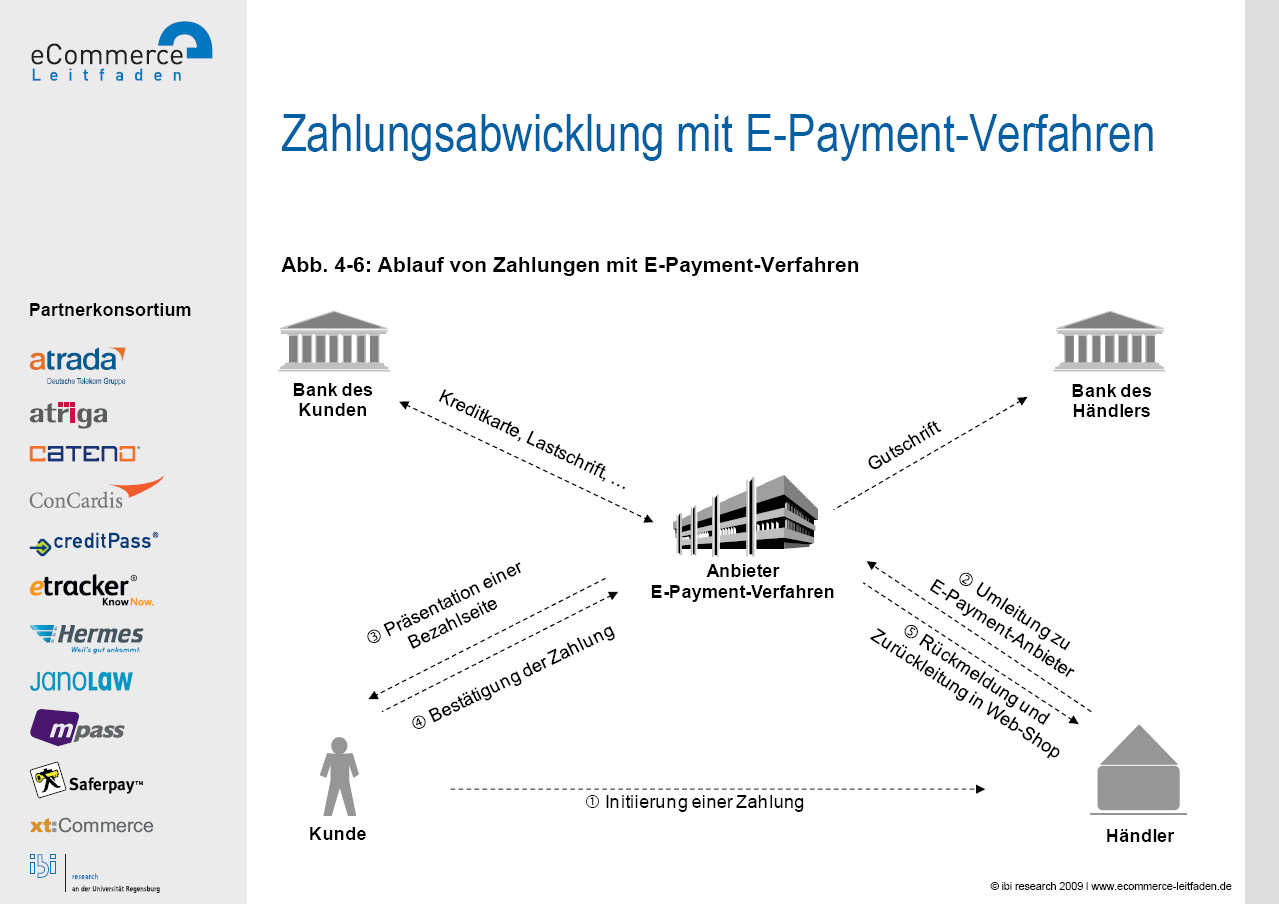
\includegraphics[width=1\linewidth]{images/zahlungsabwicklung}
	\figcaption{Zahlungsabwicklung mit elektronischen Zahlungsverfahren (src: www.ecommerce-leitfaden.de)}
\end{minipage}

Dabei wird die Bezahlung in 5 Schritte unterteilt:

\begin{enumerate}
	\item Zuerst wird die die Zahlung gestartet vom Kunden beim Händler
	\item Der Händler leitet die Anfrage zum E-Payment Anbieter um
	\item der E-Payment Anbieter präsentiert eine von sich bereitgestellte Bezahlseite
	\item Kunde bestätigt die Bezahlung
	\item E-Payment Anbieter gibt Rückmeldung an Händler
\end{enumerate}

Als nächstes werden vom E-Payment Anbieter auf die originären Zahlungsverfahren zurückgegriffen um das Geld vom Kunden anzufragen und anschließlich dem Händler gutzuschreiben. 

\subsubsection{Kategorien}
Es ist grundsätzlich in 4 große Kategorien zu unterscheiden:

\begin{itemize}
	\item E-Mail-basierte Verfahren, wie z. B. PayPal oder Moneybookers, die auf Basis von E-Mail-Adressen und -Kommunikation Zahlungsinformationen austauschen
	\item Karten-basierte Verfahren, wie z. B. die GeldKarte, paysafecard oder MicroMoney, die auf einer Karte des Anbieters des Zahlungsverfahrens basieren
	\item Mobiltelefon-basierte bzw. M-Payment-Verfahren, wie z. B. mpass oder Crandy, die den Besitz einer Mobiltelefonnummer voraussetzen und diese in den Zahlungsablauf einbinden (vgl. das Interview mit Jochen Bornemann, Vodafone, und Michael Kurz, Telefónica O2)
	\item Sonstige Inkasso- und Billing-Verfahren, wie z. B. ClickandBuy, WEB.Cent oder T-Pay, die einzelne Beträge zusammenfassen und dem Händler in einem Betrag auf ein Bankkonto auszahlen
\end{itemize}

Hierbei ist zu beachten, dass jedes Verfahren seine Vor- und Nachteile mit sich bringt und nicht definiert werden kann welches das ''Beste' ist. 

\subsubsection{Anstieg der Popularität}
Daher Online-Shopping immer beliebter wird, werden elektronische Zahlungsmittel auch immer relevanter. In Zukunft werden vor allem traditionelle Banken auch umspringen müssen auf den Trend der Vernetzung.

Zusätzlich zu beachten ist, dadurch das Firmen wie \textbf{PayPal} weit aus mehr Umsätze machen als so manche Banken, müssten diese eigentlich auch staatlich geregelt werden und Fairness für den User gewährleisten. Tatsächlich ist es momentan schon so weit dass staatliche Regelungen bei E-Payment Anbietern durchgezogen werden, aber es sei bekannt dass diese noch stärker angezogen werden.

 

	%!TEX root=../document.tex

\subsection{Kryptowährungen}
\subsubsection{Allgemeines}
\subsubsection{kek}
	\section{Ethische Fragestellungen}
Mithilfe den Schritten der ethischen Urteilsfindung wird der ethische Sachverhalt sowie die ethische Fragestellung dargestellt.

\subsection{Microtransactions}
\subsubsection{Sachverhalt}
Es ist möglich in Anwendungen, besonders im Bereich der Unterhaltung, für einen geringen Betrag sogenannte In-App-Käufe zu tätigen, welche je nach Anwendung einen kleinen Vorteil gegenüber Anderen bieten. In Applikationen, welche gezielt für Kinder entwickelt werden, wird nicht auf Microtransactions verzichtet. Moderne Zahlungssysteme ermöglichen einen einfach Ablauf der Zahlung.

\subsubsection{Fragestellung}
Ist es als Entwickler/Unternehmen in Ordnung leicht abwickelbare In-App-Käufe in Applikation für Kinder zu ermöglichen?

\subsection{Anonymität}
\subsubsection{Sachverhalt}
Es ist möglich über das Internet mithilfe von Kryptowährungen komplett anonym Geschäfte abzuwickeln. Diese Zahlungen sind erst 2 Jahre nach der Transaktion nachverfolgbar. 

\subsubsection{Fragestellung}
Sollte man anonymisierte Kryptowährungen verbieten um illegalen Bestellungen nachgehen zu können?

\subsection{Unreguliertes Zahlungssystem}
\subsubsection{Sachverhalt}
Kryptowährungen bauen ein unabhängig und vom Finanzsystem unreguliertes Zahlungssystem auf, welches nicht den staatlichen Regeln entspricht. 

\subsubsection{Fragestellung}
Sollten unabhängige und unregulierte Zahlungssysteme verboten werden, weil sie dem Finanzsystem schaden?

\section{Prüfungsfragen}

\begin{enumerate}
	\item Erläutern Sie die Schritte bei einer Zahlungsabwicklung per E-Payment
	\item Erklären Sie die ''Buchhaltung'' von Kryptowährungen
\end{enumerate}


	
	\clearpage
	
	\listoffigures
	
\end{document}
